\documentclass[a2paper, 12pt]{article}
\usepackage[font={huge, bf}]{caption}
\usepackage{fontspec}
\setmainfont{Arial}
\usepackage{subcaption}
\usepackage{graphicx}
\usepackage{tikz}
\usepackage{tikzsymbols}
\usetikzlibrary{calc,patterns,shapes.geometric}
\usepackage{float}
\usepackage{pdflscape}
\usepackage{geometry}
\geometry{landscape, margin=2cm}
\captionsetup[subfigure]{justification=justified,singlelinecheck=false}
\pagestyle{empty}

\def\centerarc[#1](#2)(#3:#4:#5){\draw[#1] ($(#2)+({#5*cos(#3)},{#5*sin(#3)})$) arc (#3:#4:#5);}

\begin{document}
	\vspace*{\fill}
	\begin{figure}[!htbp]
		\centering
		\begin{subfigure}[b]{0.48\textwidth}
			\caption{Figure 1}
			\centering
			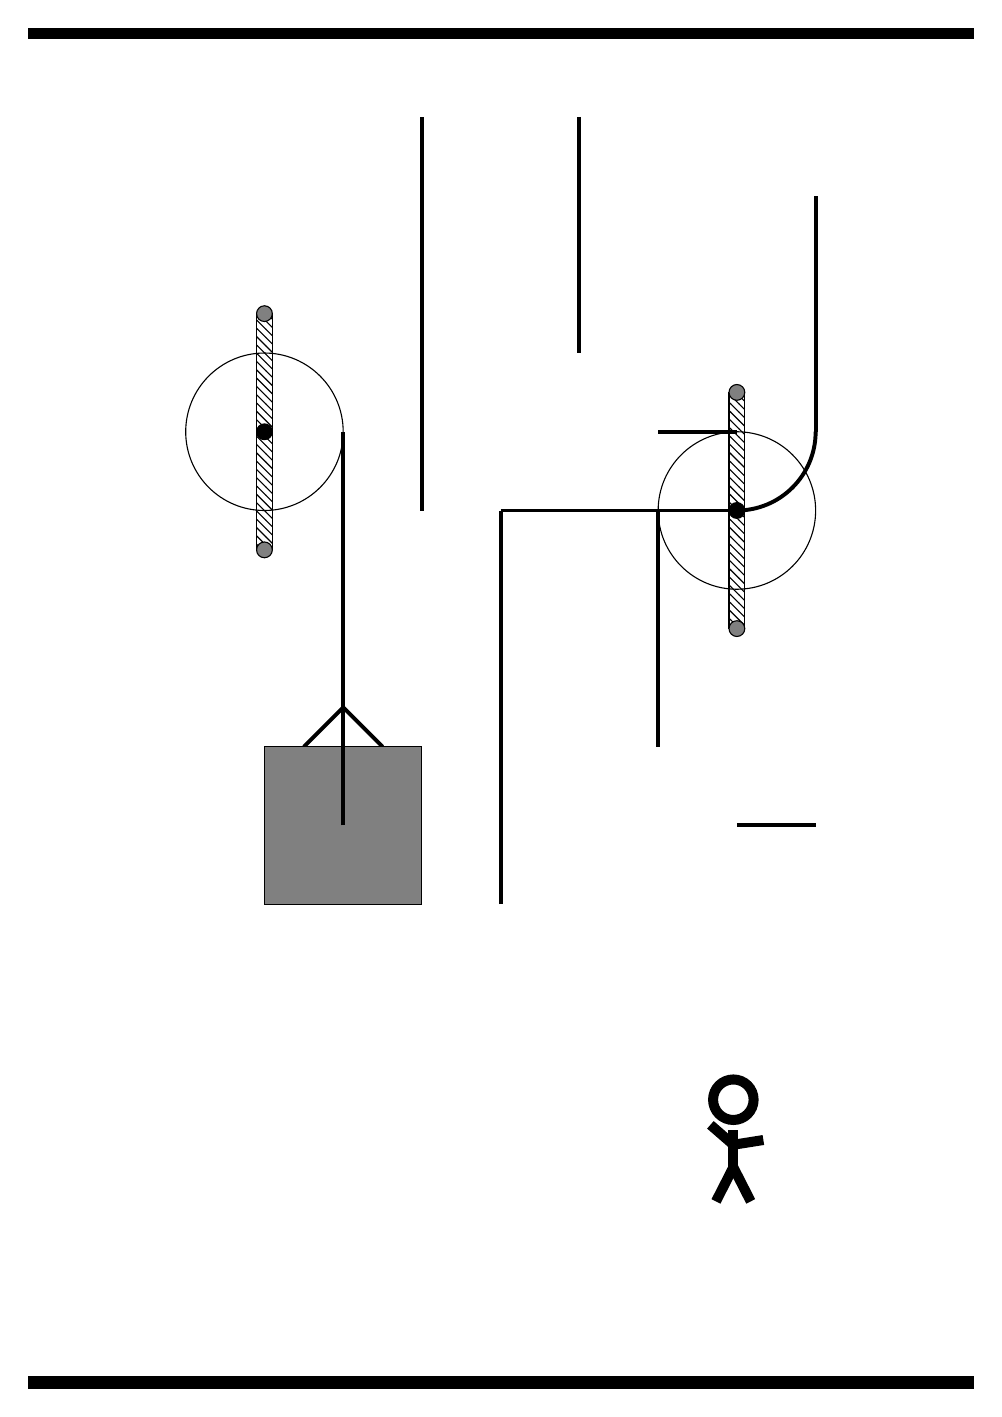
\begin{tikzpicture}
				\draw[fill=black] (-2, 14) rectangle (10, 14.125);
				
				\draw (7,8) circle (1);
				\draw[fill=black] (7,8) circle (0.1);
				\draw[pattern=north west lines, pattern color=black] (6.9,9.5) rectangle (7.1,6.5);
				\draw[fill=black!50] (7,9.5) circle (0.1);
				\draw[fill=black!50] (7,6.5) circle (0.1);
				
				\draw (1,9) circle (1);
				\draw[fill=black] (1,9) circle (0.1);
				\draw[pattern=north west lines, pattern color=black] (0.9,10.5) rectangle (1.1,7.5);
				\draw[fill=black!50] (1,10.5) circle (0.1);
				\draw[fill=black!50] (1,7.5) circle (0.1);
				
				\draw[line width=0.5mm](1.5,5) --  (2,5.5) -- (2.5,5);
				\draw[fill=black!50] (1, 5) rectangle (3, 3);
				
				\draw[line width = 0.5mm] (4,3) -- (4,8);
				\centerarc[line width = 0.5mm](5,8)(0:180:1);
				\draw[line width = 0.5mm] (6,8) -- (6,5);
				\centerarc[line width = 0.5mm](7,5)(270:180:1);
				\draw[line width = 0.5mm] (7,4) -- (8,4);
				\draw[line width = 0.5mm] (3,8) -- (3,13);
				\centerarc[line width = 0.5mm](4,13)(0:180:1);
				\draw[line width = 0.5mm] (5,13) -- (5,10);
				\centerarc[line width = 0.5mm](6,10)(270:180:1);
				\draw[line width = 0.5mm] (6,9) -- (7,9);
				\draw[line width = 0.5mm] (4,8) -- (7,8);
				\draw[line width = 0.5mm] (7,8) arc (270:360:1);
				\draw[line width = 0.5mm] (8,9) -- (8,12);
				\draw[line width = 0.5mm] (2,4) -- (2,9);
				\centerarc[line width = 0.5mm](3,9)(0:180:1);
				
				\node at (7, 0) {\scriptsize \Strichmaxerl[10][-41][9]};
				
				\draw[fill=black] (-2, -3) rectangle (10, -3.15);
			\end{tikzpicture}
		\end{subfigure}
		\hfill
		\begin{subfigure}[b]{0.48\textwidth}
			\caption{Figure 2}
			\centering
			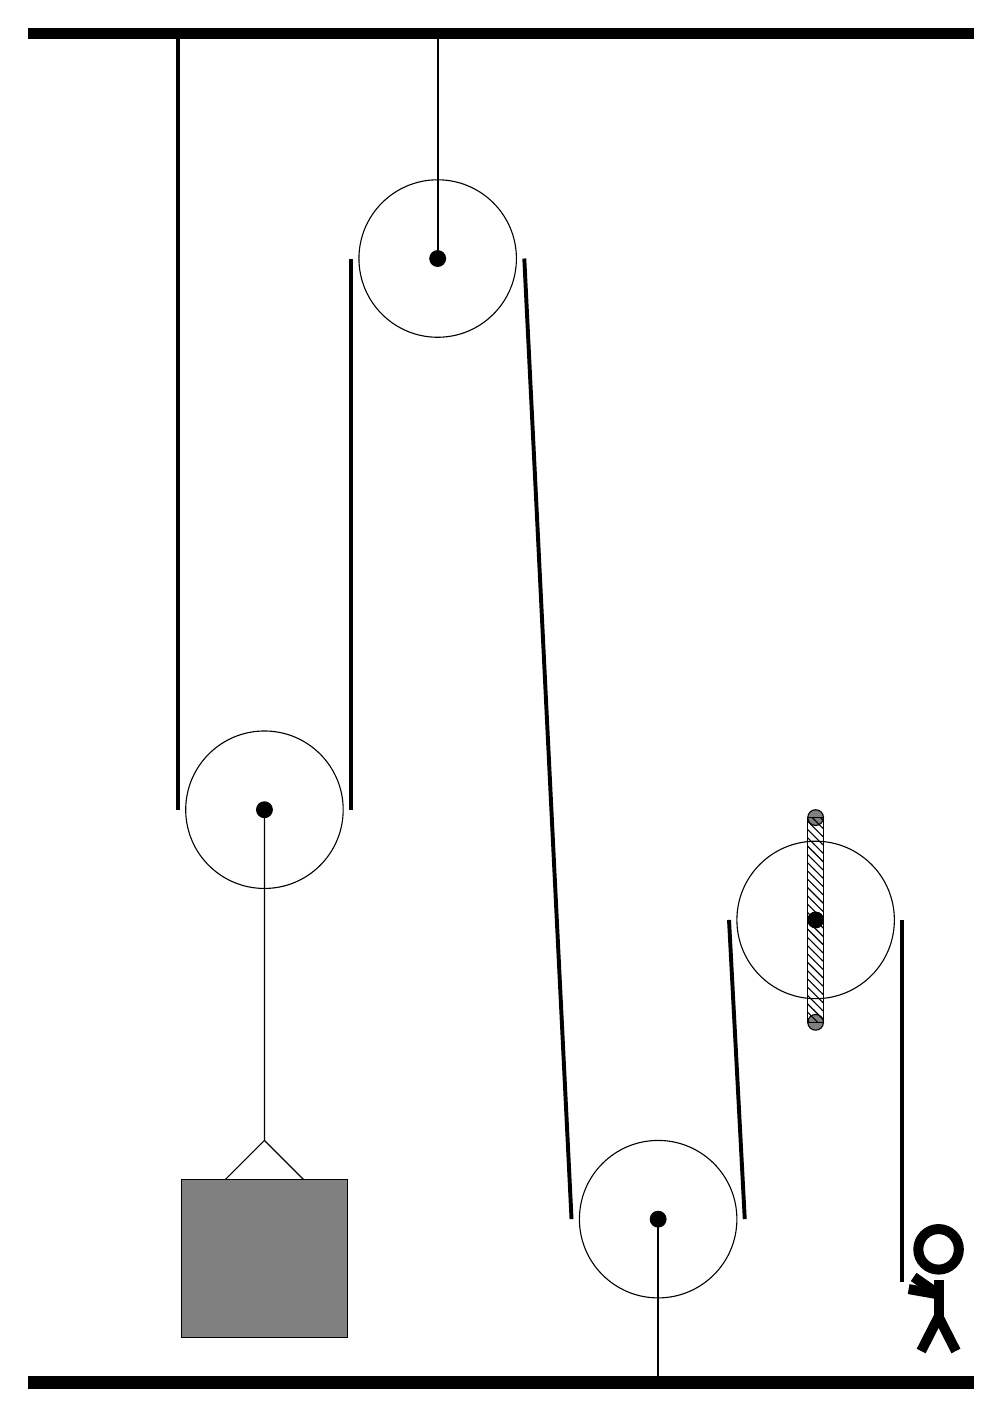
\begin{tikzpicture}
				\draw[fill=black] (-2, 14) rectangle (10, 14.125);
				
				\draw (1, 4.2) circle (1);
				\draw[fill=black] (1, 4.2) circle (0.1);
				
				\draw (3.2, 11.2) circle (1);
				\draw[fill=black] (3.2, 11.2) circle (0.1);
				\draw[thick] (3.2, 11.2) -- (3.2, 14);
				
				\draw (6, -1) circle (1);
				\draw[fill=black] (6, -1) circle (0.1);
				\draw[thick] (6, -1) -- (6, -3);
				
				\draw[fill=white](8, 2.8) circle (1);
				\draw[fill=black] (8, 2.8) circle (0.1);
				\draw[fill=black!50] (8, 4.1) circle (0.1);
				\draw[fill=black!50] (8, 1.5) circle (0.1);
				\draw[pattern=north west lines, pattern color=black] (7.9, 4.1) rectangle (8.1, 1.5);
				
				\draw (1, 4.2) -- (1, 0) -- (0.5, -0.5);
				\draw (1, 0) -- (1.5, -0.5);
				\draw[fill=black!50] (-0.05, -0.5) rectangle (2.05, -2.5);
				
				\draw[line width=0.5mm] (-0.1, 14) -- (-0.1, 4.2);
				\centerarc[line width=0.5mm](1, 4.2)(180:360:1.1);
				\draw[line width=0.5mm](2.1, 4.2) -- (2.1, 11.2);
				\centerarc[line width=0.5mm](3.2, 11.2)(0:180:1.1);
				\draw[line width=0.5mm](4.3, 11.2) -- (4.9, -1);
				\centerarc[line width=0.5mm](6, -1)(180:360:1.1);
				\draw[line width=0.5mm](7.1, -1) -- (6.9, 2.8);
				\centerarc[line width=0.5mm](8, 2.8)(0:180:1.1);
				\draw[line width=0.5mm](9.1, 2.8) -- (9.1, -1.8);
				
				\node at (9.5, -1.9) {\scriptsize \Strichmaxerl[10][-35][170]};
				
				\draw[fill=black] (-2, -3) rectangle (10, -3.15);
			\end{tikzpicture}
		\end{subfigure}
	\end{figure}
		\vspace*{\fill}
\end{document}